% !TeX encoding = UTF-8

\documentclass{protokol}


\usepackage{tikz}
\usetikzlibrary{calc}
\usetikzlibrary{arrows}

%====== Units =====
\usepackage{siunitx}
\sisetup{inter-unit-product =\ensuremath{\cdot}}
\sisetup{group-digits = integer}
\sisetup{output-decimal-marker = {,}}
\sisetup{exponent-product = \ensuremath{\cdot}}
\sisetup{separate-uncertainty}
\sisetup{tight-spacing = false}
%\sisetup{scientific-notation = true}
%\sisetup{round-mode=places,round-precision=4}
%\sisetup{evaluate-expression}


%====== Grafy =====
\usepackage{pgfplots}
\pgfplotsset{width=0.8\linewidth, compat=1.17}
\def\plotcscale{0.8}
\usepackage{pgfplotstable}
\usepackage[figurename=Obr.]{caption} % figure caption rename

%====== Rovnice align block ======
\usepackage{amsmath}
\setlength{\jot}{10pt} % rozestup mezi řádky

\graphicspath{ {./img/} }

%====== Vyplňte údaje ======
\jmeno{Jakub Charvot}
\kod{240844}
\rocnik{3.}
\obor{MET}
\skupina{MET/2}
\spolupracoval{--}

\merenodne{23.10\ 2023}
\odevzdanodne{19.10.\ 2023}
\nazev{Měření vlastností tlustovrstvých rezistorů}
\cislo{3} %měřené úlohy

\predmet{Mikroelektronika a technologie součástek}
\ustav{Ústav mikroelektroniky}
\skola{FEKT VUT v~Brně}

\def\para{x+0}
\def\parb{\para-80}


%citace 
\usepackage[backend=biber, style=iso-numeric, sortlocale=cs_CZ, autolang=other, language=czech]{biblatex}
\addbibresource{bibliography.bib}
\DeclareFieldFormat{labelnumberwidth}{\mkbibbrackets{#1}}
% hyperlinky
\usepackage[colorlinks]{hyperref}

% odstavce
\usepackage{parskip}

% Bloky kódu
\usepackage{xcolor}

%New colors defined below
\definecolor{codegreen}{rgb}{0,0.6,0}
\definecolor{codegray}{rgb}{0.5,0.5,0.5}
\definecolor{codepurple}{rgb}{0.58,0,0.82}
\definecolor{backcolour}{rgb}{0.95,0.95,0.92}

\usepackage{listings}
\lstdefinestyle{mystyle}{
  backgroundcolor=\color{backcolour}, commentstyle=\color{codegreen},
  keywordstyle=\color{magenta},
  numberstyle=\tiny\color{codegray},
  stringstyle=\color{codepurple},
  basicstyle=\ttfamily\footnotesize,
  breakatwhitespace=false,         
  breaklines=true,                 
  captionpos=b,                    
  keepspaces=true,                 
  numbers=left,                    
  numbersep=5pt,                  
  showspaces=false,                
  showstringspaces=false,
  showtabs=false,                  
  tabsize=2
}
\lstset{
	inputencoding=utf8,
	extendedchars=true,
	literate={á}{{\'a}}1 {č}{{\v{c}}}1 {ď}{{\v{d}}}1 {é}{{\'e}}1 {ě}{{\v{e}}}1 
           {í}{{\'i}}1 {ň}{{\v{n}}}1 {ó}{{\'o}}1 {ř}{{\v{r}}}1 {š}{{\v{s}}}1 
           {ť}{{\v{t}}}1 {ú}{{\'u}}1 {ů}{{\r{u}}}1 {ý}{{\'y}}1 {ž}{{\v{z}}}1 
           {Á}{{\'A}}1 {Č}{{\v{C}}}1 {Ď}{{\v{D}}}1 {É}{{\'E}}1 {Ě}{{\v{E}}}1 
           {Í}{{\'I}}1 {Ň}{{\v{N}}}1 {Ó}{{\'O}}1 {Ř}{{\v{R}}}1 {Š}{{\v{S}}}1 
           {Ť}{{\v{T}}}1 {Ú}{{\'U}}1 {Ů}{{\r{U}}}1 {Ý}{{\'Y}}1 {Ž}{{\v{Z}}}1,
	style=mystyle
	}

% Číslování
\pagenumbering{arabic}



% =========================================
% =============== DOKUMENT ================
% =========================================
\begin{document}
	%====== Vygenerování tabulky ======
	\maketitle

\section{Teoretický úvod}
  Teorie potřebná k této úloze vychází z předešlých laboratorních úloh, zejména úlohy 2, kdy jsme měřili hodnoty tlustovrstvých rezistorů v závislosti na různých podobách výpalu a také změnu jejich odporu v závislosti na teplotě. Přijde mi zbytečné uvádět znovu základní informace o samotné technologii nebo výpočtu odporu na čtverec, které již v této době semestru musí znát opravdu každý student, proto bude tato sekce o něco kratší.

\subsection{Dostavování TLV rezistorů}
Co se týče nové teorie věnuje se tato úloha také dostavování (nebo také trimmování) již natištěných rezistorů. 
Jak jsme si již vyzkoušeli na předchozích úlohách, přesnost tisku je velkou neznámou a i při optimalizaci všech dostupných parametrů jsou hodnoty stále poměrně nepřesné. Z tohoto důvodu se s nepřesností v návrhu počítá a tisknou se rezistory s o něco nižšími hodnotami než je požadováno. Následně jsou rezistory měřeny a v průběhu měření je jich část odebrána tak, aby se svou hodnotou více přiblížili požadavku. 

Nejčastějšími způsoby je mechanické osbroušení, obvykle proudem částic korundu nebo křemíku, nebo odpaření vrstvy laserem, většinou typ YAG nebo CO\(_{2}\). 

Pro dostavení je možné vyřezat do tlustovrstvého motivu různé obrazce. Obvykle se volí přímý řez od kraje směrem ke středu. Pokud se takovýchto provede více vedle a naproti sobě, vznikne serpentýnový motiv. Alternativou je ještě výřez ve tvaru L \cite{zadani,schroeder2022trimming}.

% \section{Praktická část}
% \subsection{Měření odporů čtyřbodovou metodou}
%   Čtyřbodovou metodou jsme měřili substrát č. 4. K napájení soustavy byl použit laboratorní zdroj (MATRIX MPS-3005L-3) a nastavovali jsme proud \qty{1}{\milli\ampere}, který jsme měřili a kontrolovali za pomoci digitálního multimetru (KEYSIGHT 34465A). Pro některá měření rozsah zdroje nestačil pro vytvoření tohoto proudu, měřili jsme tedy s proudem menším. 
Po nastavení proudu jsme měřili napětí druhým digitálním multimetrem (UNI-T UT804).
%   \clearpage

% \subsection{Měření teplotního koeficientu odporů -- TKR}
%   Měřili jsme teplotní závislost odporu dvou tlustovrstvých rezistorů v teplotním rozsahu 25 až \qty{140}{\degreeCelsius}. Odpor byl měřen dvojicí digitálních multimetrů (UNI-T UT805A) a teplota termočlánkem typu K. Naměřené hodnoty odporu širokého (\(R_{S} \)) a dlouhého (\(R_{D } \)) rezistoru se nachází v Tab.~\ref{tab:tkr_hodnoty}, zobrazeny jsou pak v grafu na Obr.~\ref{graf:tkr}, kde jsou také proloženy regresními přímkami. Rovnice vypočtených přímek jsou následující:
\[
    R_{S} = 2,13097-0,0000512435\cdot t
\]
\[
    R_{D} = 0,0113403\cdot t +96,2776
\]

TKR pak můžeme z těchto rovnic vyčíst následovně:
\[
    TKR_{S} = \frac{-0,0000512435}{2,13097}\cdot 100 \doteq \qty{-2,404e-3}{\percent}
\]

\[
    TKR_{D} = \frac{0,0113403}{96,2776}\cdot 100 \doteq \qty{1,178e-2}{\percent}
\]

Pro široký rezistor nám vyšel TKR negativní a naopak pro dlouhý rezistor vyšel TKR pozitivní.

\begin{table}[h!]
    \caption{Naměřené hodnoty odporů pro rostoucí teploty.}
    \centering
    \def\arraystretch{1.4}
    \begin{tabular}{l|l|l}
        \(t\)\ [\unit{\degreeCelsius}]  &   \(R_{S} \)\ [\unit{\kilo\ohm}]       &   \(R_{D} \)\ [\unit{\kilo\ohm}] \\
        \hline \hline
        25  &   2,1319  &   96,580   \\ \hline
        30  &   2,1305  &   96,667   \\ \hline
        35  &   2,1300  &   96,724   \\ \hline
        40  &   2,1299  &   -    \\ \hline
        45  &   2,1210  &   -    \\ \hline
        50  &   2,1288  &   -    \\ \hline
        55  &   2,1280  &   -    \\ \hline
        60  &   2,1294  &   96,948   \\ \hline
        65  &   2,1277  &   96,989   \\ \hline
        70  &   2,1275  &   97,024   \\ \hline
        75  &   2,1273  &   97,094   \\ \hline
        80  &   2,1273  &   97,158   \\ \hline
        85  &   2,1269  &   97,212   \\ \hline
        90  &   2,1263  &   97,278   \\ \hline
        95  &   2,1260  &   97,338   \\ \hline
        100 &   2,1257  &   97,408   \\ \hline
        105 &   2,1251  &   97,469   \\ \hline
        110 &   2,1249  &   97,533   \\ \hline
        115 &   2,1249  &   97,586   \\ \hline
        120 &   2,1249  &   97,621   \\ \hline
        125 &   2,1246  &   97,715   \\ \hline
        130 &   2,1244  &   97,769   \\ \hline
        135 &   2,1244  &   97,847   \\ \hline
        140 &   2,1243  &   97,892   \\ 
    \end{tabular}
    \label{tab:tkr_hodnoty}
\end{table}

\begin{figure*}[h!]
    \begin{tikzpicture}
        \centering
        \begin{axis}
            [
            xlabel={\( t\ [\unit{\degreeCelsius}]\)},
            ylabel={\( R\ [\unit{\kilo\ohm}]\)},
            axis y line*=left, % dve y osy
            width=1\textwidth,
            height = 0.5\textwidth,
            % legend pos=north west
            legend style={at={(0.03,0.5)},anchor=west}
%			xmin=0,
%			ymin=0,
%			xmax=100
%			ymax=100
            ]

            \addplot[mark=x, mark options={solid}, thick,  red, only marks, mark size=3pt] table [skip first n=0, x=tep, y=s, col sep=comma] {data/tkr.csv};
            
            \addlegendentry{Široký}

            \addplot [domain=20:140, smooth, thin, dashed, red] { 2.13097-0.0000512435*x};
            \addlegendentry{Regrese}
            
           
        \end{axis}   
     
        \begin{axis}
            [
            ylabel={\( R\ [\unit{\kilo\ohm}]\)},
            axis x line=none,
            axis y line*=right,
            width=1\textwidth,
            height = 0.5\textwidth,
            % legend pos=north east,
            legend style={at={(1-0.03,0.5)},anchor=east}
%			xmin=0,
%			ymin=0,
%			xmax=100
%			ymax=100
            ]

            \addplot[mark=x, mark options={solid}, thick,  blue, only marks, mark size=3pt] table [skip first n=0, x=tep, y=d, col sep=comma] {data/tkr.csv};
            
            \addlegendentry{Dlouhý}
            
            \addplot [domain=20:140, smooth, thin, dashed, blue] { 0.0113403*x+96.2776};
            \addlegendentry{Regrese}
        
    \end{axis}
        
    \end{tikzpicture}
    \caption{Teplotní závislost dvou TLV rezistorů.}
    \label{graf:tkr}
\end{figure*}


%   \clearpage

% \subsection{Výkonové zatížení odporu}
%   Postupně jsme testovali čtyři vzorky rezistorů a to konkrétně jejich výkonovou zatížitelnost v závislosti na použitém substrátu. Na laboratorním zdroji (TTi QPX1200SP) jsme nastavili napětí \qty{7}{V} a přibližně odečetli také odebíraný proud, pro všechny vzorky to bylo \qty{0,06}{A}. Vzorky pokryté termoemisní barvou jsme následně pozorovali termokamerou (FLUKE) a po ustálení stavu, tedy při maximální dosažené teplotě, jsme hodnoty zaznamenali. Porovnání jednotlivých měření se nachází na Obr.~\ref{fig:termo-png}.

\begin{figure}[h!]
    \centering
    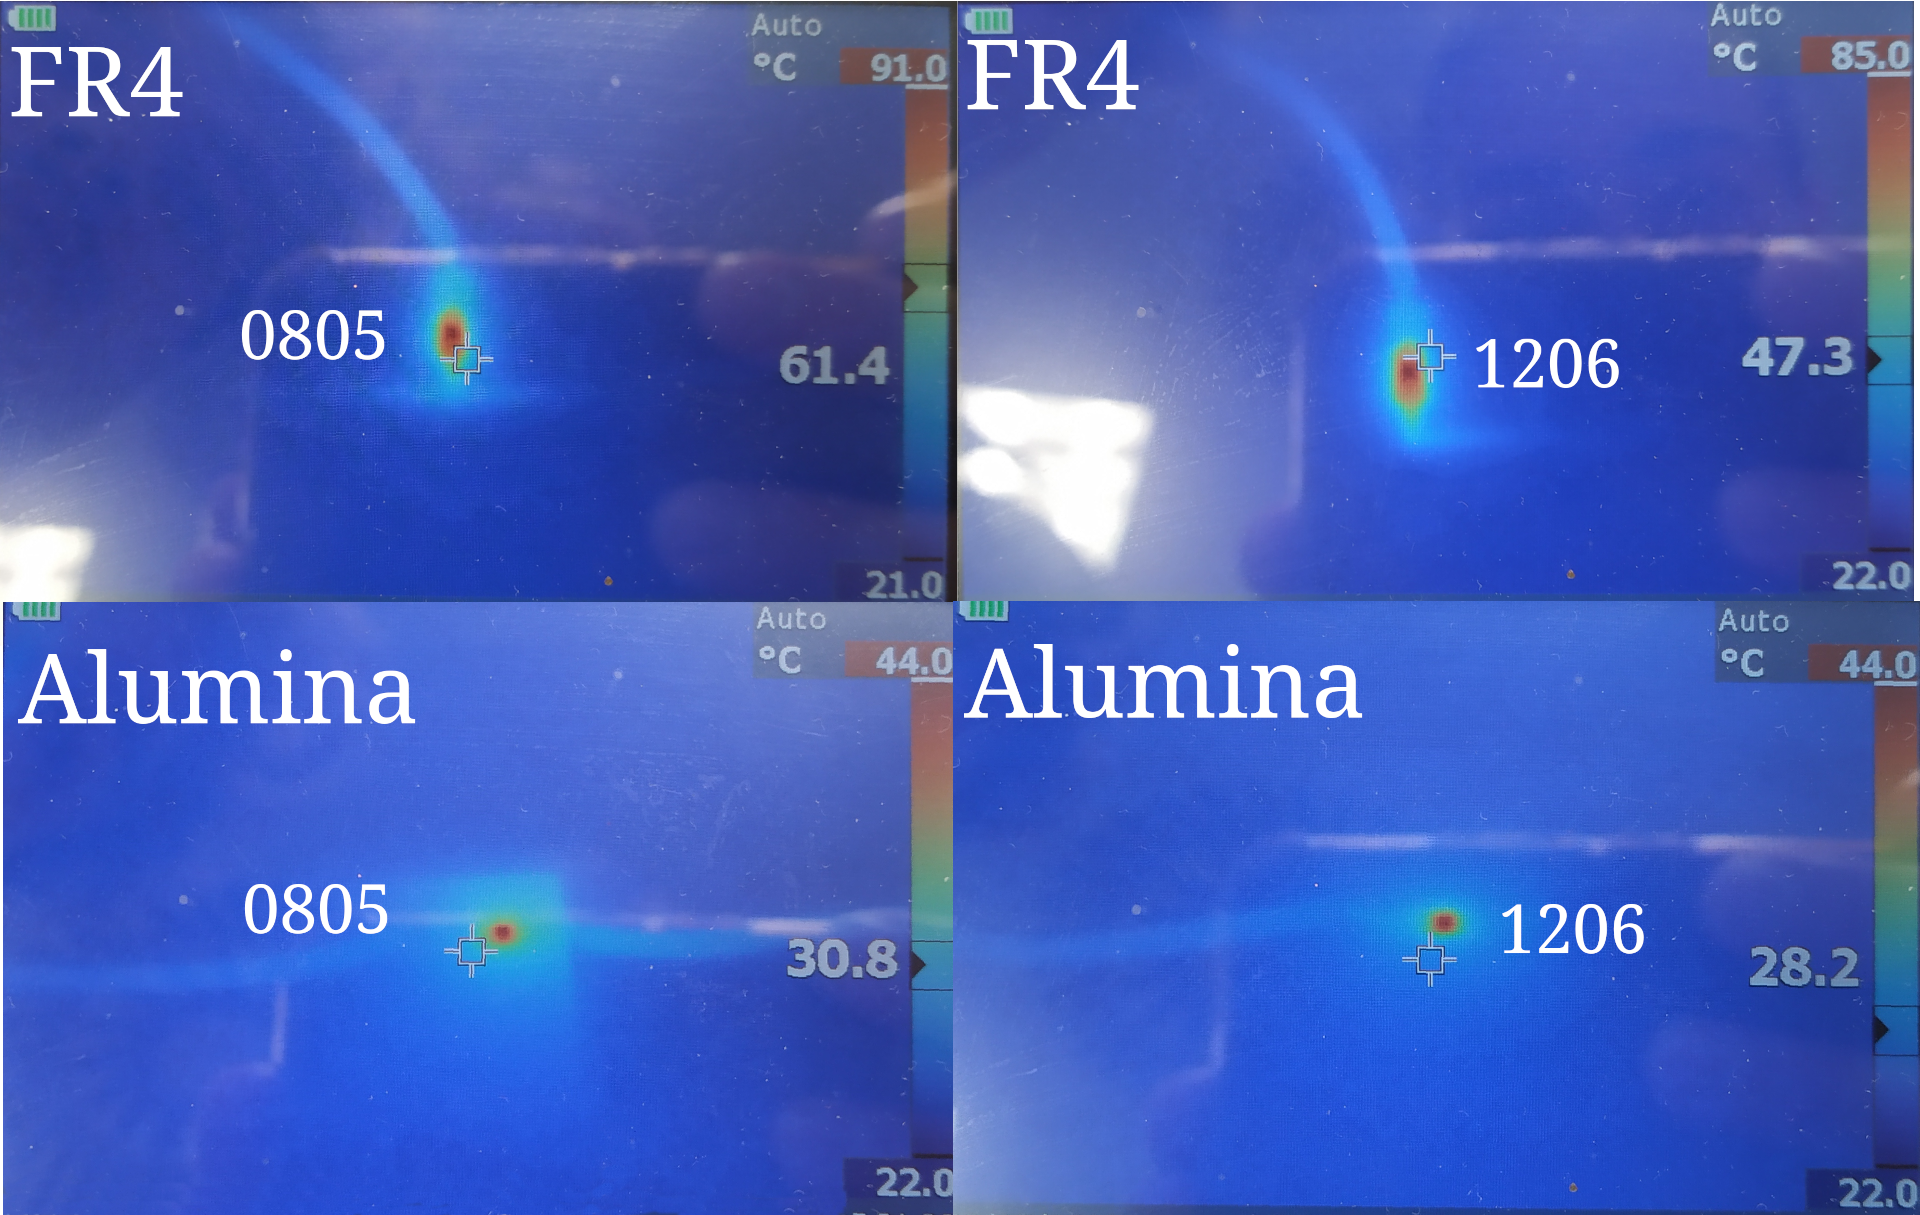
\includegraphics[width=0.8\textwidth]{termo.png}
    \caption{Porovnání ohřevu SMD rezistorů pouzder 0805 a 1206 na různých substrátech.}
    \label{fig:termo-png}
\end{figure}

Ve druhé části byl proveden destruktivní test SMD rezistoru. Zvyšováním napětí na laboratorním zdroji dochází k nárustu procházejícího proudu, ohřevu rezistoru a následně tepelnému poškození a zničení celé součástky. Výsledek testu je zobrazen na Obr.~\ref{fig:destrukce-png}. Průbeh zkoušky popisuje Tab.~\ref{tab:popis_destrukce}.

\begin{table}[h!]
    \caption{Průběh destruktivního testu SMD rezistoru.}
    \centering
    \def\arraystretch{1.4}
    \begin{tabular}{l|l}
        U\ [V] &  Popis situace \\ \hline  \hline
            12,5 &  rezistor syčí \\ \hline
            14,3 &  odpařování tavidla \\ \hline
            22,2 &  nečitelný popisek \\ \hline
            24,7 &  zvýšený zápach \\    \hline
            25,6 &  viditelné žhavé místo \\ \hline
            26,9 &   spálení součástky \\ 
    \end{tabular}
    \label{tab:popis_destrukce}
\end{table}


\begin{figure}[h!]
    \centering
    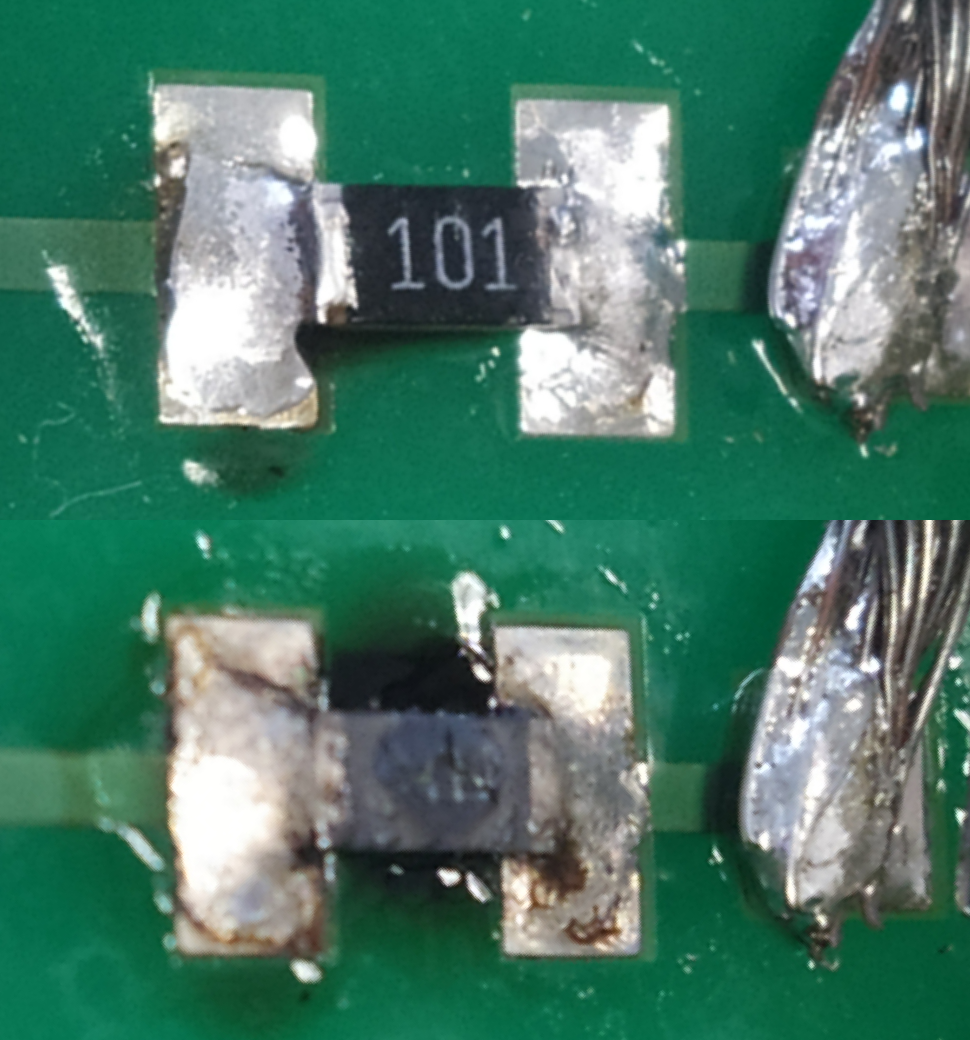
\includegraphics[width=0.8\textwidth]{destrukce.png}
    \caption{Destrukční test SMD rezistoru.}
    \label{fig:destrukce-png}
\end{figure}


%   \clearpage

\section{Závěr}
  Jak je vidět z grafů a tubulky naměřených hodnot, pro některé série jsou výsledky v různých kvadrantech obdobné, pro některé naopak vůbec. Nejhomogennějšíh výsledku dosáhla série RX\_3. Také je vidět, že napříč sériemi vycházely celkově o něco menší hodnoty v prvním kvadrantu a naopak vyšší ve druhém a třetím. 

Při porovnání naměřených hodnot s teoretickými se ale dostáváme do prekérní situace. Odchylka zde dosahuje několika řádů kdy namísto stovek \unit{\ohm} měříme hodnoty i v nižších stovkách \unit{\mega\ohm}, typycky pak v jednotkách \unit{\mega\ohm}. Toto nasvědčuje buďto hrubé systematické chybě měření neno špatným informacím ohledně použité odporové pasty, popř. kombinaci obou faktorů. Vzhledem k tomu, že měření bylo prováděno poměrně dlouhý čas a dohlíženo čtyřmi osobami se mi takto hruhá chyba jeví jako nepravděpodobná, ovšem vyloučna není. 
  
\clearpage
\section*{Reference}
\printbibliography[heading=none]

\end{document}